
\documentclass[11pt]{article}
\usepackage{standalone}
\usepackage[margin=0.75in, headheight=20pt]{geometry}

\usepackage{amsmath}
\usepackage{amsfonts}
\usepackage{amssymb}
\usepackage{mathtools}

\usepackage{caption,tabularx,booktabs}

\usepackage{rotating}

\usepackage[utf8]{inputenc}
\usepackage[english]{babel}
\setlength{\parindent}{2em}
\setlength{\parskip}{.25em}
\renewcommand{\baselinestretch}{1.0}

\usepackage{fancyhdr}
\pagestyle{fancy}
\rhead{ Clarke | Blostein | Queen's University}
\renewcommand{\headrulewidth}{0.4pt}
\renewcommand{\footrulewidth}{0.4pt}

\usepackage{courier}

\usepackage[]{algorithm2e}
\usepackage{mathrsfs}

\usepackage{etoolbox}
\patchcmd{\thebibliography}{\chapter*}{\section*}{}{}




\title{Performance Analysis of Semi-Orthogonal User Groups}
\author{J.E. Clarke, Dr. S.D. Blostein | Queen's University}
\date{Summer, 2018}

\begin{document}
	\maketitle
	\newpage
    \section{Maximum Ratio Transmission Beamforming Performance as a Function of a Known Orthogonality Requirement}
    	\subsection{System model}
            
\begin{figure}
    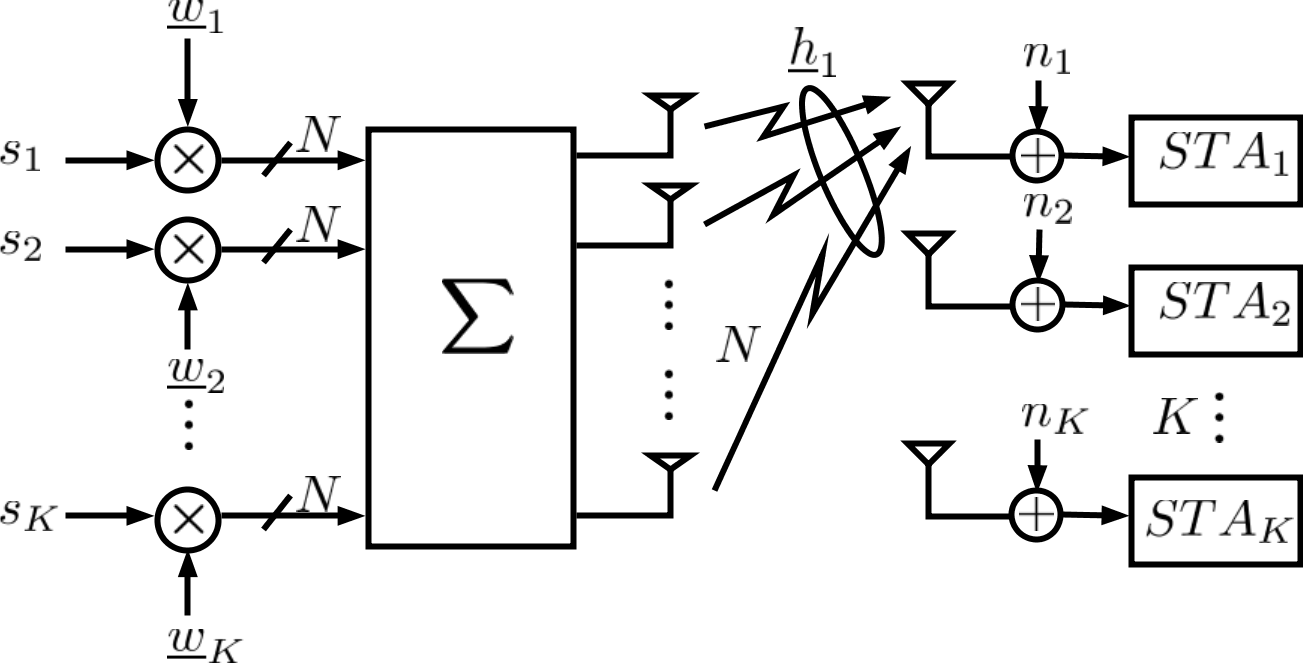
\includegraphics[width=12cm]{figs/system_desc.png}\\
    \caption{Block diagram of the system model.}
    \label{fig:sys_bd}
\end{figure}

        \subsection{Probability of SUS group existence}
            In this section we discuss a more formal definition of how STAs are grouped. It is assumed that the $K$ STAs shown in Fig. \ref{fig:sys_bd} are selected according to constraints or requirements placed on orthogonality between STAs, and the magnitude of the channel norm of a given STA. A finite number of STAs are considered for addition to the group. By only considering a finite number of STAs for addition to the group, we can express the probability that we can form a group of a given size that meet orthogonality and channel norm constraints \cite{Swannack2005}. 

The requirement for an $\epsilon$-orthogonal group (semi-orthogonal STA selection group, or SUS group) is broken into two parts. Firstly the STAs in the group are required to have a channel norm similar to other STAs in the group. The upper and lower bound on SNR ensures that STAs in an SUS group have similar large-scale channel gains. Asserting an upper and lower bound can be viewed a coarse form of power control. 

The second requirement deals with interference between STAs in an SUS group. Once it has been determined that a given STA meets the SNR requirement, then it is compared against other candidate STAs to ensure interference is sufficiently low. The inner product between a STA's channel and other candidate STA's channels is formed. The magnitude of the product is compared to a threshold , $\epsilon$. If the product is lower than the threshold, STAs are said to be $\epsilon$-orthogonal and the STAs are added to the SUS group.
 \begin{equation}\label{eq:S_e}
    \begin{aligned}
        \mathcal{S}_\epsilon = \lbrace \mathcal{S}_a \big|\ | \underline{h_i}^H\underline{h_j} |\ <\ \epsilon \ \text{;} \ \rho^-<\Vert \underline{h_i} \Vert^2 < \rho^+\ \forall \ i \neq j \in \mathcal{S}_a \rbrace
    \end{aligned}
\end{equation}
Where $\mathcal{S}_a$ is the set of all STAs within service range of the AP, and $\mathcal{S}_\epsilon$ is a collection of $\epsilon$-orthogonal SUS group of length $L$.

Based on this expression, we ultimately want to arrive at a probability that an SUS group exists: $Pr[\mathcal{S}_\epsilon \neq \lbrace \emptyset \rbrace]$. A lower bound on $Pr[\mathcal{S}_\epsilon \neq \lbrace \emptyset \rbrace]$ based on these requirements is developed in \cite{Swannack2005}. Probability of SUS group existence depends on the orthogonality requirements given in Eq. (\ref{eq:S_e}), the group size $K$ , and the number of candidate STAs considered for addition to the SUS group, $L$. 

The CDF of the channel norm will be denoted by $F_{\Vert\underline{hi}\Vert^2}(m,\rho)$, where $\rho$ are realizations of the random variable formed by the channel norm. Each term in the $N$-length vector, $\underline{h}_i$ is represented by two normal random variables: one for the real part and one for the imaginary part. When forming the L2 norm of the $N$-length vector, each multiplication forms a sum of length four where each of the arguments of the sum are a product of two random variables. Namely, the sum takes the form real$\cdot$real + real$\cdot$imaginary + imaginary$\cdot$real + imaginary$\cdot$imaginary. Thus, the CDF expression becomes:

\begin{equation}\label{eq:ch_sq_cdf_chan}
    \begin{aligned}
        F_{\Vert\textbf{hi}\Vert^2}(\rho;m)& = \Gamma_n(2m,m\rho)\\
        &= Pr[\Vert\textbf{h}_i\Vert^2 \leq \rho]
    \end{aligned}
\end{equation}

The probability that the channel satisfies SNR requirements, namely that $\Vert\underline{h}_i\Vert^2$ lands in the shell between radii $\rho^+,\ \rho^-$,  is given by the subtraction of the respective CDF expressions:
\begin{equation}\label{eq:p_s}
    \begin{aligned}
        p_s = \Gamma_n(2N,N\rho^-) - \Gamma_n(2N,N\rho^+)
    \end{aligned}
\end{equation}

The conditional probability that the orthogonality requirement is met, given that the channel norm falls between $\rho^-$ and $\rho^+$, $p_\perp$, is lower bounded as follows:
\begin{equation}\label{eq:p_perp}
    \begin{aligned}
        p_\perp &\geq (1-(K-l)\delta_c(\theta_{\epsilon,\rho},2N))^{K-1}\\
        where:\\
        \theta_{\epsilon,\rho} &= \arccos\frac{\epsilon}{\rho}
    \end{aligned}
\end{equation}

The function $\delta_c(\theta,2m)$ is motivated by a sphere packing approach. It is defined as the ratio of the area of a spherical (polar) caps of a sphere in $2m$ dimensions formed by $\theta$ to the entire surface area of the sphere:
\begin{equation}\label{eq:delta_c_sphere}
    \begin{aligned}
        \delta_c(\theta,2N) = 2\frac{\Omega_{2N}(\theta)}{\Omega_{2N}(\pi)}
    \end{aligned}
\end{equation}

A lower bound for $\delta_c(\cdot)$ is given by:
\begin{equation}\label{eq:delta_c_lbnd}
    \begin{aligned}
        \delta_c(\theta,2N) &\geq c(\theta;s,\beta)\ \ \text{if}: \ s = \frac{\pi}{2\psi_{N-2}} \ and \ \beta \geq N-1\\
        where:\\
        c(\theta;s,\beta) &\triangleq \bigg(\frac{2}{\pi}\theta\bigg)^s\sin^\beta\theta\\
        \psi_N &\triangleq \frac{\sqrt{\pi}}{N}\frac{\Gamma(\frac{N+1}{2})}{\Gamma(\frac{N}{2})}
    \end{aligned}
\end{equation}

The expression that an SUS group of at least size $K$ will exist within a  pool of $L$ candidate STAs is lower bounded by:
\begin{equation}\label{eq:p_exist}
    \begin{aligned}
        Pr_\epsilon = Pr[\vert \mathcal{S}_\epsilon \vert > 0] &\geq Pr[M_\rho \geq K] - c_1 ( 1 + p_s (e^{-E(p_\perp,K)} -1 ))^L\\
        where:\\
        E(p,K) &\triangleq \text{max}\bigg \lbrace \frac{2p^2}{K},\frac{8p}{25K}\big(\frac{K-1}{e\cdot K}\big)^{K-1}\bigg \rbrace \\
        c_1 &=  \begin{cases}
                    \text{exp}(\frac{2p_\perp^2(K-1)}{K}), & \text{if } E(p_\perp,K) = \frac{2p_\perp^2}{K}, \\
                    1, & \text{otherwise}.
                \end{cases}\\
        Pr[M_\rho \geq K]&= \sum_{j=K}^{L}\binom{L}{j}p_s^j (1-p_s)^{L-j}
    \end{aligned}
\end{equation}
Derivations and proofs of $\delta_c(\cdot), P_\epsilon$ are length, and, therefore, will not be regurgitated here. Please refer to \cite{Swannack2005}, \cite{SwannackThesis} for such proofs.
        \subsection{MRT beamforming , SINR, and sum rate analysis}\label{sec:linear_sinr}
            A maximum ratio transmission (MRT) scheme is utilized for determining the transmission beamforming vectors, $\underline w_i,\ i = 1,2,\ldots K$. MRT is based on maximizing the signal-to-noise ratio (SNR)--it neglects interference. The SNR for $STA_i$ is given by:
\begin{equation}
     \begin{aligned}\label{eq:snr}
        SNR_i &= \frac{\vert \underline{h_i}^H \underline w_i \vert^2}{\sigma_n^2}\\
        &= \frac{\vert \underline{h_i}^H \Tilde{\underline w_i} \vert ^2 P_i}{\sigma_n^2}
     \end{aligned}
 \end{equation}
 By the Cauchy-Schwarz inequality, we know that $SNR_i$ is maximized when the channel vector and the beamforming vector are in the same direction, thus maximizing the magnitude of their inner product. Therefore, we let $\underline w_i^{\star} = \underline h_i$ for MRT beamforming. The direction of the MRT beamforming vector becomes $\Tilde{\underline w_i}^{\star} = \frac{\underline{h_i}}{\Vert h_i \Vert}$.
 
 The the upper bound for the SNR, which is achieved by using an MRT beamforming scheme, is given by:
 \begin{equation}
     \begin{aligned}\label{eq:snr_mrt}
            SNR_i^{\star} &= \frac{\vert \underline{h_i}^H \frac{\underline{h_i}} {\Vert \underline{h_i} \Vert} \vert ^2 P_i}{\sigma_n^2}\\
            &= \frac{\Vert \underline{h_i}\Vert^2 P_i}{\sigma_n^2}
     \end{aligned}
 \end{equation}
 
 We now consider interference to develop an expression for SINR that makes use of the MRT scheme. It is important to notice the MRT scheme does not mitigate the effects of interference. The MRT scheme is a special case of a more general beamforming scheme that does not neglect interference (as one might expect). A method for arriving at such a beamforming scheme is discussed at some length in \cite{Bjornson2014}. An MRT scheme is assumed here for the sake of practical simplicity. The SINR is an extension of the SNR given in Eq. (\ref{eq:snr_mrt}) that can be realized by observing the structure of the expanded receive signal given in Eq. (\ref{eq:rx_sig_expanded}).
  \begin{equation}
     \begin{aligned}\label{eq:sinr_mrt}
            SINR_i^{\star} &=  \frac{\Vert \underline{h_i}\Vert^2 P_i}{\sum_{j \neq i}^K \vert \frac{\underline{h_i}^H\underline{h_j}}{\Vert \underline{h_j}\Vert}\vert^2 P_j + \sigma_n^2}
     \end{aligned}
 \end{equation}
 
 Observe from Eq. (\ref{eq:sinr_mrt}) that the interference term in the denominator is in the form of an inner product between two channel vectors. This inner product term can be interpreted as a measure of orthogonality between the two stochastic channel vectors. Consider comparing this term to the orthogonality requirement in Eq. (\ref{eq:S_e}).

The upper and lower bounds on the SNR are used to approximate the power allocated to each beamforming vector. Since the channel norms are bounded, we approximate that each beamforming vector the same amount of power allocated to it. That is, the total power is evenly divided amongst each of the beamforming vectors: $P_i = \frac{P_{tot}}{N}\ \forall i=1,2\ldots K$.

We can make substitutions to Eq. (\ref{eq:sinr_mrt}) that incorporate SUS orthogonality and channel norm requirements from \ref{eq:S_e}.
\begin{equation}\label{eq:sinr_epsilon}
    \begin{aligned}
        SINR_i^{\star} &=  \frac{\Vert \underline{h_i}\Vert^2 \frac{P_{tot}}{N}} {\epsilon^2 \frac{P_{tot}}{N} \sum_{j \neq i}^K  \frac{1}{\Vert \underline{h_j}\Vert^2} + \sigma_n^2}
    \end{aligned}
\end{equation}

It is worth-while reiterating that channel norms follow a Gamma distribution: $\Vert \underline{h_i} \Vert^2 , \Vert \underline{h_j} \Vert^2 \sim \mathcal{G}(2N,\frac{2}{N})$. Therefore, the expression given in Eq. (\ref{eq:sinr_epsilon}) is valid at a given instant in time. The fading channel is assumed to be fast with respect to symbol transmit period. Ergodicity is assumed, and the statistical mean of Shannon capacity is calculated by taking the arithmetic mean with a sufficiently large number of samples and equating it to the statistical mean. There is further elaboration on this point in the experiment implementation discussion dealing with Monte Carlo analysis. The instantaneous Shannon capacity conditioned on SUS group existence is given by:
\begin{equation}\label{eq:capacity}
    \begin{aligned}
        C_i^{\star} \ \vert \ [Pr_\epsilon = 1] &= \log_2(1 + SINR_i^{\star})\ \text{bps/Hz}
    \end{aligned}
\end{equation}

The conditional sum rate for the SUS group is given by:
\begin{equation}\label{eq:sum_rate_conditional}
    \begin{aligned}
        C^{\star} \ \vert \ [Pr_\epsilon = 1] &= \sum_{i=1}^K C_i^{\star}  \ \vert \ [Pr_\epsilon = 1]
    \end{aligned}
\end{equation}

It is important to note here that only one SUS group receives data at any given time. For example, if there are four transmit antennas, and there are two STAs only two STAs receive service. Two of the transmit antennas are unused, and only one SUS group of two STAs receives service at a given time. It is also worth while to note that the no weighting scheme that encourages fairness is used.

The expression in Eq. (\ref{eq:capacity}) is conditioned on the fact that the SUS group exists. In the context of this experiment, there are a finite number of STAs available to the AP. Moreover, a finite subset of these STAs are considered for addition to a given SUS group in order to limit channel sounding overhead. Therefore, it is not guaranteed that an SUS group will exist. Furthermore, the probability that an SUS group exists, $P_{\epsilon}$, may be expressed in terms of the parameters $\epsilon,\rho^-,\rho_+$, in Eq. (\ref{eq:S_e}), and the number of candidate STAs considered for addition to the SUS group \cite{Swannack2005}. The expressions used for $Pr_\epsilon$ are lengthy, and the same as those used in \cite{Swannack2005}. It is left to the reader to refer to \cite{Swannack2005} for details regarding this probability. Thus, the unconditional sum rate is given by:
The conditional sum rate for the SUS group is given by:
\begin{equation}\label{eq:sum_rate}
    \begin{aligned}
        C^{\star} &=  (C^{\star} \ \vert \ [Pr_\epsilon = 1])\cdot Pr_\epsilon
    \end{aligned}
\end{equation}







        \subsection{MRT beamforming , SINR, and sum rate analysis for single-dimensional constellations}\label{sec:wl_sinr}
            The expressions in Section \ref{sec:linear_sinr} assume a two-dimensional constellation for transmitted symbols. In order to arrive at the Shannon capacity expression in Eq. (\ref{eq:capacity}), symbols are chosen from a continuous alphabet that follows a circularly symmetric complex normal distribution. In this section we discuss similar expressions in the context of a single-dimensional constellation rather than a two-dimensional constellation (ie. a real modulation scheme such as M-PAM rather than a complex modulation scheme such as M-QAM).

Although the transmitted symbols are real-valued in this case, processing will still be performed in the complex domain. However, since the data is only being modulated onto real parts of the signals being processed, we can no longer model signals as proper random variables. To handle, this impropriety, we employ widely linear processing techniques \cite{Adali2011}.

First we consider relaxing the orthogonality and SNR constraints, by limiting  requirements to only the real part of the channel inner product and norm.  Let the  transformation, $\mathcal{T}$, be the transformation of the complex vector in $\mathbb{C}^N$ to a real vector in $\mathbb{R}^{2N}$:
\begin{equation}\label{eq:complex_real_xform}
    \begin{aligned}
        \underline{h_i} \in \mathbb{C}^N \xrightarrow{\mathcal{T}} \hat{\underline{h}}_i = [ \mathfrak{Re} \lbrace \underline{h}_i \rbrace \ \mathfrak{Im}\lbrace \underline{h}_i \rbrace ] \in \mathbb{R}^{2N}
    \end{aligned}
\end{equation}
Thus,
\begin{equation}\label{eq:orth_real_transp}
    \begin{aligned}
        \mathfrak{Re} \lbrace \underline{h}_i^H\underline{h}_j \rbrace = \hat{\underline{h}}_i^T \hat{\underline{h}}_j 
    \end{aligned}
\end{equation}

Following from Eqs. (\ref{eq:S_e},\ref{eq:orth_real_transp}) the relaxed expression for the collection of SUS groups becomes:
\begin{equation}\label{eq:wl_S_e}
    \begin{aligned}
        \mathcal{S}_{\epsilon,\mathfrak{R}} = \lbrace \mathcal{S}_a \big|\  \hat{\underline{h}}_i^T \hat{\underline{h}}_j<\ \epsilon \ \text{;} \ \rho^-<\Vert \hat{\underline{h}}_i \Vert^2 < \rho^+\ \forall \ i \neq j \in \mathcal{S}_a \rbrace
    \end{aligned}
\end{equation}

For the relaxed SNR requirement,the Gamma distribution used to derive the expression in (\ref{eq:p_s}), now only has 2$m$ degrees of freedom, rather than 4$m$ degrees of freedom since the inner product form a sum of 2$m$ real components. Therefore the expression for relaxed probability the norm will fall in the shell defined by radii $\rho^-,\rho^+$, $p_{s,\mathfrak{R}}$ becomes:
\begin{equation}\label{eq:p_s_real}
    \begin{aligned}
        p_{s,\mathfrak{R}} = \Gamma_n(m,m\rho^-) - \Gamma_n(m,m\rho^+)
    \end{aligned}
\end{equation}

The increase in dimensions from $N \rightarrow 2N$ also changes the the arguments of $\delta_c(\theta_{\epsilon,\rho},2N)$ in Eq. (\ref{eq:p_perp}) to $\delta_c(\theta_{\epsilon,\rho},4N)$.
\begin{equation}\label{eq:p_perp_real}
    \begin{aligned}
        p_{\perp,\mathfrak{R}} &\geq (1-(K-l)\delta_c(\theta_{\epsilon,\rho},4N))^{K-1}\\
        where:\\
        \theta_{\epsilon,\rho} &= \arccos\frac{\epsilon}{\rho}
    \end{aligned}
\end{equation}

The expression for SUS group existence probability remains the same as Eq. (\ref{eq:p_exist}) substituting the necessary values for $p_s,p_\perp$. The widely linear existence probability is given by $Pr_{\epsilon,\mathfrak{R}}$.

In order to make a fair comparison between single-dimonsional and two-dimensional constellation schemes in terms of sum rate, the capacity of the single-dimensional scheme must be scaled by a factor of two since there are now only half as many bits per symbol. Therefore the unconditional sum rate for a single-dimensional constellation scheme is given by:
\begin{equation}\label{eq:sum_rate_real}
    \begin{aligned}
        C^{\star}_\mathfrak{R} &=  \frac{1}{2}(C^{\star} \ \vert \ [Pr_{\epsilon,\mathfrak{R}} = 1])\cdot Pr_{\epsilon,\mathfrak{R}}
    \end{aligned}
\end{equation}

        \subsection{Experiment Implementation}
            A Monte Carlo simulation was performed in order to determine the ergodic sum rate. The sum rate was simulated according to Eqs. (\ref{eq:sum_rate},\ref{eq:sum_rate_real}) for $n_T$ independent trials. The values of each independent trial were then averaged together to determine the ergodic sum rate. The ergodic sum capacity is calculated as follows.
\begin{equation}\label{eq:erg_sum_rate}
    \begin{aligned}
    \overline{C^\star} = \sum_{t=1}^{n_T} C_t^\star
    \end{aligned}
\end{equation}
Where $t$ is the index of the independent Monte Carlo trials.

A 95\% confidence interval is assumed for all simulations. The magnitude of the error on the estimated data point from the Monte Carlo simulation is given by:
\begin{equation}\label{eq:ebar_mag}
    \begin{aligned}
    \vert E_{bar} \vert = \Phi^{-1}\bigg(1-\frac{1-0.95}{2}\bigg)\frac{s}{\sqrt{n_T}}
    \end{aligned}
\end{equation}
Where $\Phi (\cdot)$ is the CDF for a normal distribution, and  $s = \sqrt{\frac{\sum_{t=1}^{n_T}(C_t^\star-\overline{C^\star})^2}{n_T-1}}$ is the arithmetic standard deviation of the trials. 

Constant and variable parameters of the simulations are shown in Table \ref{tab:exp_param}: left-hand table shows parameters that are constant for all simulations, the right-hand table shows parameters that vary depending on the simulation. 
\captionof{table}{Constant (left) and variable (right) experiment parameters} \label{tab:exp_param}
\begin{tabular}{ p{1.25cm}  p{4cm}  p{2cm} }\toprule[1.5pt]
\bf Symbol & \bf Description & \bf Value \\\midrule
$P_{tot}$ & Total transmit power & 1 W\\
$N$ & Number of transmit antennas & 4\\
$\sigma_n^2$ & AWGN power & 100 mW\\
$\rho^-$ & SNR requirement lower bound & 1\\
$\rho^+$ & SNR requirement upper bound & 2\\
$n_{T}$ & Number of Monte Carlo trials & 200\\
\bottomrule[1.25pt]
%$0$ & $0$\\
\end{tabular}
\quad
%\captionof{table}{Variable Parameters} \label{tab:var_param}
\begin{tabular}{ p{1.25cm}  p{4cm} }\toprule[1.5pt]
\bf Symbol & \bf Description \\\midrule
$\epsilon$ & SUS group orthogonality requirement \\
$K$ & SUS group size \\
$\vert \mathcal{S}_a \vert$ & Number of candidate STAs considered for SUS group \\
\bottomrule[1.25pt]
%$0$ & $0$\\
\end{tabular}
\setlength{\parindent}{2em}
\setlength{\parskip}{.25em}
\renewcommand{\baselinestretch}{1.0}

        \subsection{Results}
            
Results are shown from two sets of simulations in Figs. \ref{fig:15_candidate},\ref{fig:30_candidate}. Both of these figures show sum rate given in Eq. (\ref{eq:erg_sum_rate}) plotted vs. $\epsilon$. The left-hand side of the plots corresponds to more strict orthogonality (small $\epsilon$), while the right-hand side of the plot corresponds to more lax orthogonality (larger values of $\epsilon$)

The results shown in Fig. \ref{fig:15_candidate} are for $L = 15$. Results illustrated in this plot are broken into series that vary depending on $K$ and dimension of symbol constellation. The colour and shape of the datapoints in the series denotes the value of $K$: blue triangle for $K=2$, red square for $K=3$, and black circle for $K=4$. The fill of the datapoint denotes the dimension of constellation used for symbols: no fill corresponds to single dimensional (real) constellation (ie. BPSK, M-PAM), while solid fill corresponds to a two-dimensional (complex) constellation (ie. QPSK, M-QAM).

First we will discuss the data series belonging to two-dimensional constellations. From the plot we can see that there is a point of maxima for $0 < \epsilon < \infty$ in each of these curves. The location of this point of maxima agrees with expected results. The shape of these curves illustrates a tradeoff associated with choosing $\epsilon$: $\epsilon$ is best chosen such that it provides some degree of orthogonality between users to limit interference; however, it should not be so strict that we cannot find STAs to add to the SUS group that meet the orthogonality requirement. The portion of the curve to the left of the maximum is limited in terms of SUS group existence. The portion of the curve to the right of the maximum is limited in terms of interference. We can see that the curves with higher values of $K$ have a maximum associate with larger values of $\epsilon$ since we have a lower probability of finding a large number of STAs that meet strict orthogonality requirements. We can see that even though we are twice as many STAs with $K=4$ compared to $K=2$, the maximal sum rate is higher for $K=2$ than $K=4$. Although this result may seem counter-intuitive, consider the constraints being placed on these curves in terms of SUS group existence probability and interference. For $K=4,\ L = 15$ by the time existence probability is high enough to stop limiting sum rate, interference is high enough to limit the achievable sum rate below the $K=2$ case.

Next, consider the series corresponding to single-dimensional constellations. From these series we can see that lower values of $\epsilon$ are favorable. This is because the relaxed orthogonality requirement translates to a higher probability of SUS group existence, even for strict orthogonality requirements. We see  that the series for $K=4$ now has the largest maximum sum rate. Again, this is expected. Since the probability of SUS group existence has been significantly relaxed compared to the two-dimensional constellation case, the $K=4$ series is able to have a large enough existence probability at low interference to out-perform the $K=2$ series.

\begin{sidewaysfigure}
    \centering
    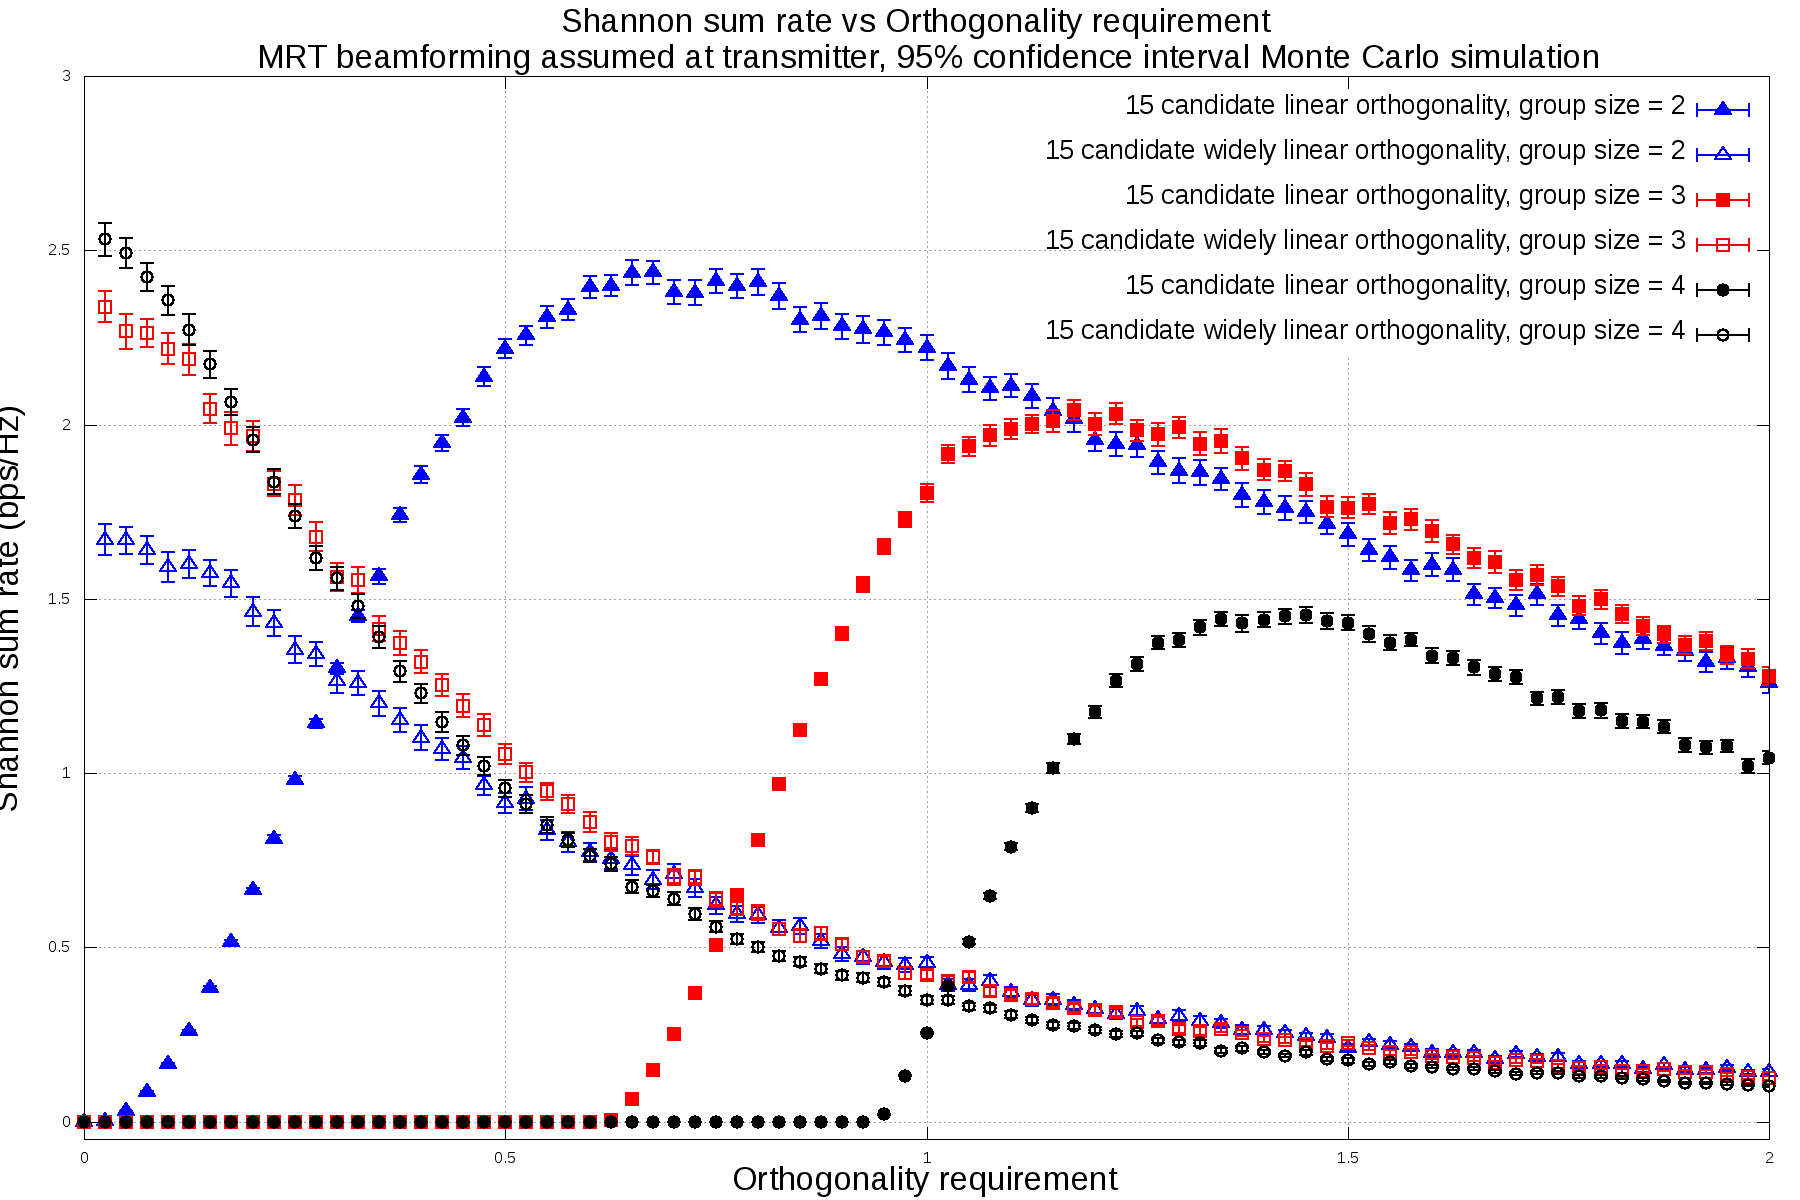
\includegraphics[width=24cm]{figs/15_candidate_mrt.png}\\
    \caption{Sum rate for single-dimensional and two-dimensional constellations, SUS group sizes set to 2, 3, 4. Number of candidate STAs for addition to SUS groups is held to 15.}
    \label{fig:15_candidate}
\end{sidewaysfigure}

Figure \ref{fig:30_candidate} shows  curves for two-dimensional constellation sum rates with $L = 30$ instead of 15. We see that the $K=3,4$ series now have higher maximum sum rate values. This result is expected: as the number of candidate STAs is increased, the probability of larger SUS groups existing for small values of $\epsilon$ increases. Increasing $L$ has less of an impact for $K=2$ because the existence probability has already saturated for small values of $\epsilon$.
\begin{sidewaysfigure}
    \centering
    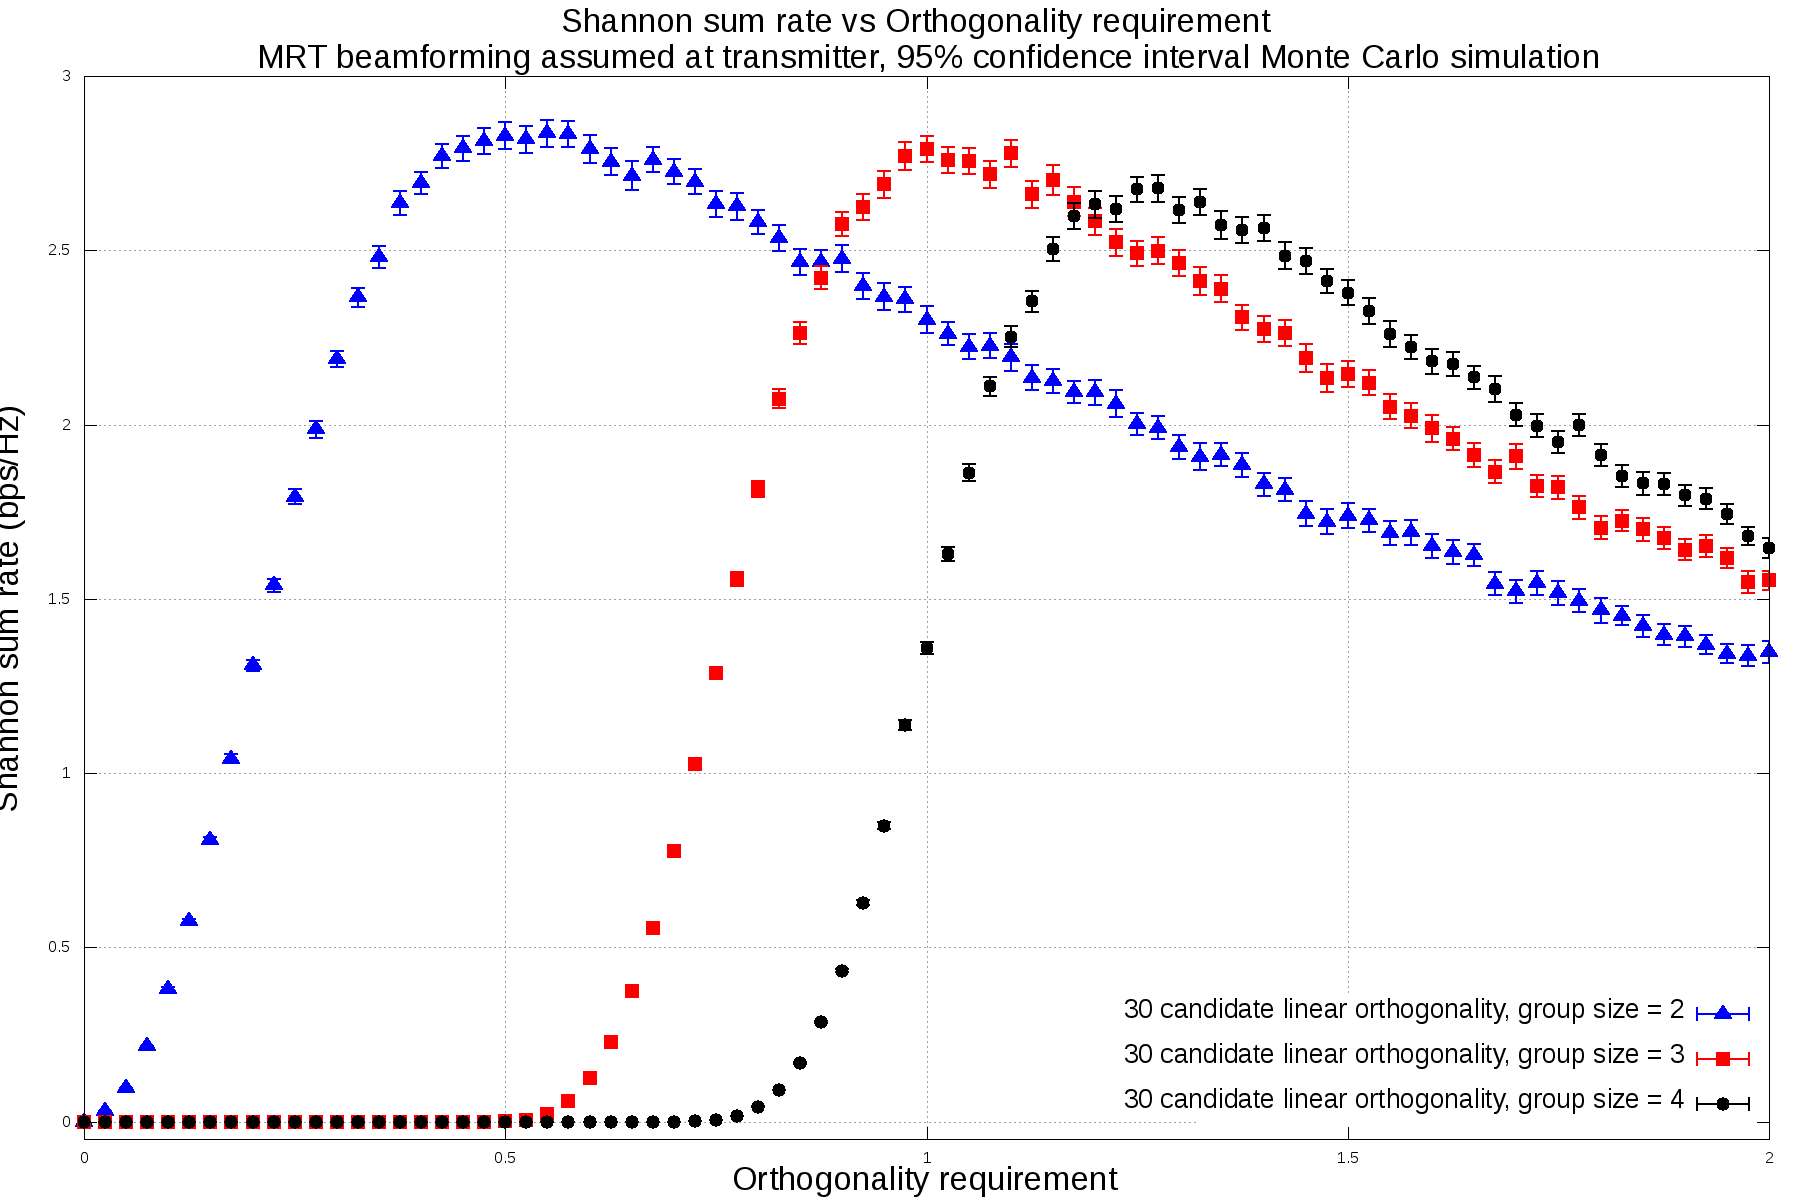
\includegraphics[width=24cm]{figs/30_candidate_mrt.png}\\
    \caption{Sum rate for two-dimensional constellations, SUS group sizes set to 2, 3, 4. Number of candidate STAs for addition to SUS groups is held to 30.}
    \label{fig:30_candidate}
\end{sidewaysfigure}


    \newpage
    \section{Maximum Ratio Transmission Beamforming Performance, Estimating Orthogonality Requirement}
    WORKING ON IT... :)
	%\section{Appendices}
	    %\subsection{Notes on Gamma-distributed variables}
	    %    \input{app/gamma_dist.tex}
    \newpage	
 	\begingroup
 		\renewcommand{\section}[2]{}%
 		\bibliographystyle{IEEEtran}
 		\bibliography{references}
 	\endgroup
\end{document}

Imported from Another project/review.tex, at 3:21 pm Today

 
